\documentclass[12pt, A4]{article}
\usepackage[utf8]{inputenc}
\usepackage{geometry}
\geometry{
	a4paper,
	left=15mm,
	right=15mm,
	top=25mm,
	bottom=20mm
}
\usepackage{graphicx}
\graphicspath{ {./images/} }
\usepackage{amsmath}
\usepackage{amsfonts}
\usepackage{amssymb}
\usepackage{hyperref}
\usepackage{amsthm}
\hypersetup{
	colorlinks=true,
	linkcolor=black,
	filecolor=magenta,      
	urlcolor=cyan,
	pdfpagemode=FullScreen,
}

\makeatletter

\newtheorem*{remark}{Remark}

\renewcommand{\theenumi}{\roman{enumi}}

\newcommand{\indep}{\perp \!\!\! \perp}

\newcommand{\sq}{$\square$}
\newcommand{\rmk}{$\surd$}
\newcommand{\trick}{$\bigstar$}
\newcommand{\N}{\mathbb{N}}
\newcommand{\R}{\mathbb{R}}
\newcommand{\U}{\mathcal{U}}
\newcommand{\V}{\mathcal{V}}
\newcommand{\A}{\mathcal{A}}
\newcommand{\B}{\mathcal{B}}
\newcommand{\C}{\mathcal{C}}
\newcommand{\G}{\mathcal{G}}
\newcommand{\F}{\mathcal{F}}
\newcommand{\LL}{\mathcal{L}}
\newcommand{\open}{\underset{open}{\subset}}
\newcommand{\closed}{\underset{closed}{\subset}}
\newcommand{\subsp}{\underset{subsp}{\subset}}
\newcommand{\seq}{\underset{seq}{\subset}}
\newcommand{\cl}{\overline}
\newcommand{\diff}{\,\backslash\,}
\newcommand{\union}{\,\cup\,}
\newcommand{\intersect}{\,\cap\,}
\newcommand{\exist}{\exists\,}
\newcommand{\convp}{\overset{P}{\rightarrow}}
\newcommand{\convd}{\overset{D}{\rightarrow}}
\newcommand{\foranyn}{\quad \forall \, n\in \N}

\begin{document}
\begin{titlepage}
	\begin{center}
		\vspace*{5cm}
		\textbf{\Large Probability theory \MakeUppercase{\romannumeral 2} Assignment 1}
		\\
		\vspace{1.5cm}
		\textbf{2021-21116 Taeyoung Chang}
		\vfill
		Exercises in Section 4.1 Conditional Expectation
		\\
	
		\vspace*{3cm}
		\thispagestyle{empty}
	\end{center}
\end{titlepage}
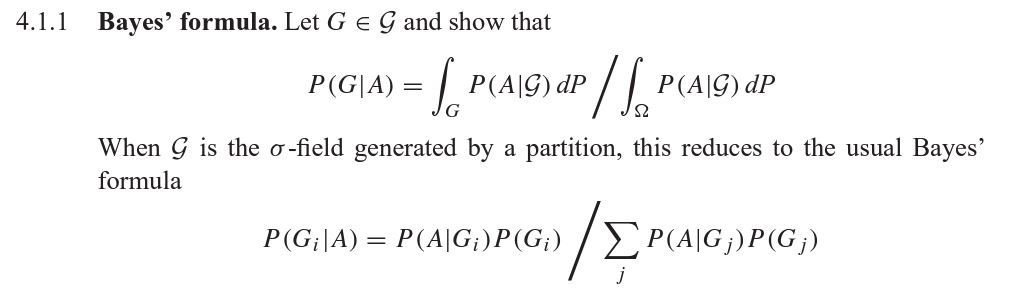
\includegraphics{Exer4.1.1.JPG}
\begin{remark}
    We didn't define `conditional prob. given a set' in the lecture, but in the textbook, the author said that ``To continue the connection with undergraduate notions, $P(A|B):=P(A\intersect B)\,/\,P(B)$''
\end{remark}
\begin{proof}
    $P(G|A)=P(G\intersect A)/P(A)$. Note that $P(A|\G)=E[I_A|\G]$
    \begin{align*}
        \int_G P(A|\G)\, dP &=\int_G E[I_A|\G]\,dP=\int_G I_A\, dP=P(A\intersect G) \\ \int_\Omega P(A|\G)\, dP &= \int_\Omega E[I_A|\G]\,dP=\int_\Omega I_A\, dP =P(A)
    \end{align*}
    The second equality in each of two equations above is due to the definition of conditional expectation and the fact that $G, \Omega \in \G$. Therefore the equaltiy $P(G|A)=\int_G P(A|\G)\, dP / \int_\Omega P(A|\G)\, dP$ holds true. To prove the equation for Bayes' formula, we shall use a lemma learned in the lecture.
	\\ (Lemma) $\Omega=\bigcup_{i=1}^\infty \Omega_i$ is a partition of $\Omega$ with $\Omega_i\in \F_0$ and $P(\Omega_i)>0\quad \forall \, i\in \N$ \\$\F=\sigma\{\Omega_1, \Omega_2,\cdots\}=\{\bigcup_{j\in \kappa} \Omega_j : \kappa\subset \N\}$ \quad ($\F$ is a $\sigma$-field). \quad Then we have 
	$$ E[X|\F]=\sum_{i=1}^\infty a_i I_{\Omega_i} \quad with \quad a_i=\frac{E[XI_{\Omega_i}]}{P(\Omega_i)}$$
	Now, $\G=\sigma\{G_1,G_2,\cdots\}$ with $\Omega=\bigcup_{i=1}^\infty G_i$ is a partition. 
	\begin{align*}
		\int_{G_i} P(A|\G)\,dP &= \int_{G_i} E[I_A|\G]\,dP \underset{lemma}{=} \int_{G_i} \sum_{j=1}^\infty \frac{E[I_A I_{G_j}]}{P(G_j)} I_{G_j}\,dP \underset{MCT}{=} \sum_{j=1}^\infty \int_{G_i}\frac{E[I_{A\intersect G_j}]}{P(G_j)} I_{G_j}\,dP \\ &\underset{partition}{=} \int_{G_i} \frac{P(A\intersect G_i)}{P(G_i)}\cdot 1\,dP = P(A|G_i) P(G_i) \\
		\int_{\Omega} P(A|\G)\,dP &= \int_{\Omega} E[I_A|\G]\,dP \underset{lemma}{=} \int_{\Omega} \sum_{j=1}^\infty \frac{E[I_A I_{G_j}]}{P(G_j)} I_{G_j}\,dP \underset{MCT}{=} \sum_{j=1}^\infty \int_{\Omega}\frac{E[I_{A\intersect G_j}]}{P(G_j)} I_{G_j}\,dP \\ &= \sum_{j=1}^\infty \int_{G_j} \frac{P(A\intersect G_j)}{P(G_j)}\cdot 1\,dP = \sum_{j=1}^\infty P(A|G_j) P(G_j) 
	\end{align*}
	Therefore the equality $P(G_i|A)=P(A|G_i)P(G_i) \,/\, \sum_j P(A|G_j)P(G_j)$ holds true.
\end{proof}
\clearpage

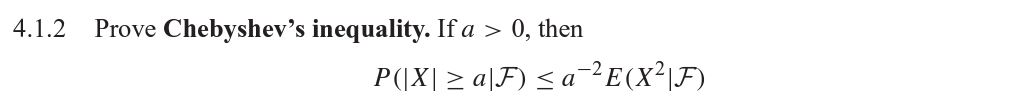
\includegraphics{Exer4.1.2.JPG}
\begin{proof}
	\begin{align*}
		P( |X|\geq a\, |\, \F)&=E[I(|X|\geq a)|\F] = E[I(X^2\geq a^2)|\F]\leq E\Big[\frac{X^2}{a^2}I(X^2\geq a^2)|\F\Big]\\ &= \frac{1}{a^2}E[X^2I(X^2\geq a^2)|\F]\leq \frac{1}{a^2}E[X^2|\F]
	\end{align*}
\end{proof}
\vspace{1cm}


\includegraphics{Exer4.1.3.JPG}
\begin{proof}
	Take arbitrary $a\in \R$. Assume $E[X^2],\, E[Y^2]<\infty$
	\begin{align*}
		0&\leq E[(aX+Y)^2 |\G]=a^2E[X^2|\G]+2aE[XY|\G]+E[Y^2|\G]\\ &= E[X^2|\G]\Big(a+\frac{E[XY|\G]}{E[X^2|\G]} \Big)^2+E[Y^2|\G]-\frac{E^2[XY|\G]}{E[X^2|\G]}
	\end{align*}
	Since the inequality above holds for any $a\in \R$, $E[Y^2|\G]-\frac{E^2[XY|\G]}{E[X^2|\G]}\geq0$ must hold, which implies that $E^2[XY|\G]\geq E[X^2|\G]E[Y^2|\G]$
\end{proof}
\vspace{1cm}


\includegraphics{Exer4.1.5.JPG}
\begin{proof}
	Set two $\sigma$-fields $F_1,\, F_2\subset \mathcal{P}(\Omega)$  as below : 
	\begin{align*}
		\F_1 &=\sigma(\{a\})= \big\{\phi, \{a\}, \{b,c\}, \{a,b,c\}\big\} \\ \F_2 &= \sigma(\{c\})= \big\{\phi, \{c\}, \{a,b\}, \{a,b,c\}\big\}
	\end{align*}
	$\F_0:=\mathcal{P}(\Omega)$. $\F_1$ and $\F_2$ are sub $\sigma$-fields of $\F_0$. Define $X : \Omega \rightarrow \R$ by $X(a)=0,\; X(b)=1, \; X(c)=0$ \\ $$(X\geq k) = \begin{cases}
		\phi \in \F_0 & if\quad k>1 \\ \{b\}\in \F_0 & if\quad 0<k\leq 1 \\  \{a,b,c\}\in \F_0 & if\quad k\leq 0 
	\end{cases}$$ $X$ is a $F_0$-measurable random variable. Notice that $X$ is neither $\F_1$-measurable, nor $\F_2$-measurable. Also, we shall define probabiliy measure $P$ on $(\Omega, \F_0)$ by $P(\{a\})=P(\{b\})=P(\{c\})=1/3$\\
	Our strategy for the proof is that find out $E[X|\F_1]$ and $E[E[X|\F_1]|\F_2]$ in order, and then claim that it is not $\F_1$-measurable so that it cannot be equal to $E[E[X|\F_2]|\F_1]$.\\
	\begin{enumerate}
		\item Find out $E[X|\F_1]$\\
		In $\F_1$, unlike in $\F_0$, $\{b\}$ and $\{c\}$ cannot be separated. Since $P(\{b\})=P(\{c\})=1/3$ and \\$(X(b)+X(c))/2=1/2$, we can guess that $Y$ defined by $Y(a)=0, \; Y(b)=1/2,\; Y(c)=1/2$ might be $E[X|\F_1]$. 
		$$(Y\geq k) = 
		\begin{cases}
			\phi \in \F_1 & if\quad k>1/2 \\ \{b,c\}\in \F_1 & if \quad 0<k\leq 1/2 \\  \{a,b,c\}\in \F_1 & if\quad k\leq 0 
		\end{cases}$$
		Hence $Y$ is $\F_1$-measurable.
		\begin{align*}
			\int_\phi X\, dP &= 0	 &	 \int_{\{b,c\}} X\, dP&= 0\cdot P(\{b\})+1\cdot P(\{c\})=1/3   \\
			 \int_{\{a\}} X\, dP&= 0\cdot P(\{a\})=0	&	 \int_{\{a,b,c\}} X\,dP &=0\cdot P(\{a\})+1\cdot P(\{b\})+0\cdot P(\{c\})=1/3 \\
			 \int_\phi Y\, dP &= 0	 &	 \int_{\{b,c\}} Y\, dP&= 1/2\cdot P(\{b\})+1/2\cdot P(\{c\})=1/3   \\
			 \int_{\{a\}} Y\, dP&= 0\cdot P(\{a\})=0	&	 \int_{\{a,b,c\}} Y\,dP &=0\cdot P(\{a\})+1/2\cdot P(\{b\})+1/2\cdot P(\{c\})=1/3 
		\end{align*}
		Thus $\int_A X\, dP=\int_A Y\, dP \quad \forall \, A\in \F_1$. \quad $Y=E[X|\F_1]\; a.s.$
		
		\item Find out $E[E[X|\F_1]|\F_2]$\\
		In $\F_2$, $\{a\}$ and $\{b\}$ cannot be separated. Since $P(\{a\})=P(\{b\})$ and $(Y(a)+Y(b))/2=1/4$, we can guess that $Z$ defined by $Z(a)=1/4, \; Z(b)=1/4, \; Z(c)=1/2$ might be $E[Y|\F_2]=E[E[X|\F_1]|\F_2]$.
		$$(Z\geq k) = 
		\begin{cases}
			\phi \in \F_2 & if\quad k>1/2 \\ \{c\}\in \F_2 & if \quad 1/4<k\leq 1/2 \\  \{a,b,c\}\in \F_2 & if\quad k\leq 1/4 
		\end{cases}$$
		Hence $Z$ is $\F_2$-measurable.
		\begin{align*}
			\int_\phi Y\, dP &= 0	 &	 \int_{\{a,b\}} Y\, dP&= 0\cdot P(\{a\})+1/2\cdot P(\{b\})=1/6   \\
			 \int_{\{c\}} Y\, dP&= 1/2 \cdot P(\{c\})=1/6	&	 \int_{\{a,b,c\}} Y\,dP &=0\cdot P(\{a\})+1/2 \cdot P(\{b\})+1/2\cdot P(\{c\})=1/3 \\
			 \int_\phi Z\, dP &= 0	 &	 \int_{\{a,b\}} Z\, dP&= 1/4\cdot P(\{a\})+1/4\cdot P(\{b\})=1/6   \\
			 \int_{\{c\}} Z\, dP&= 1/2\cdot P(\{c\})=1/6	&	 \int_{\{a,b,c\}} Z\,dP &=1/4 \cdot P(\{a\})+1/4\cdot P(\{b\})+1/2\cdot P(\{c\})=1/3 
		\end{align*}
		Thus $\int_A Y\,dP=\int_A Z\, dP \quad \forall \, A\in \F_2$. \quad $Z=E[Y|\F_2]=E[E[X|\F_1]|\F_2]$
		
		\item Conclusion \\
		Observe that $Z$ is not $\F_1$-measurable. This is because $(Z\geq k)=\{c\}\notin \F_1$ whenever $1/4<k\leq 1/2$. Suppose $E[E[X|\F_1]|\F_2] = E[E[X|\F_2]|\F_1]\; a.s.$. Then since $P(\{a\})=P(\{b\})=P(\{c\})=1/3 >0$, \; $E[E[X|\F_2]|\F_1]=Z$ (exactly same). This means that $E[E[X|\F_2]|\F_1]$ is not $\F_1$-measurable, which is a contradiction. \\ Therefore, $E[E[X|\F_1]|\F_2] \neq E[E[X|\F_2]|\F_1]$ in this case.
	\end{enumerate}
\end{proof}
\clearpage

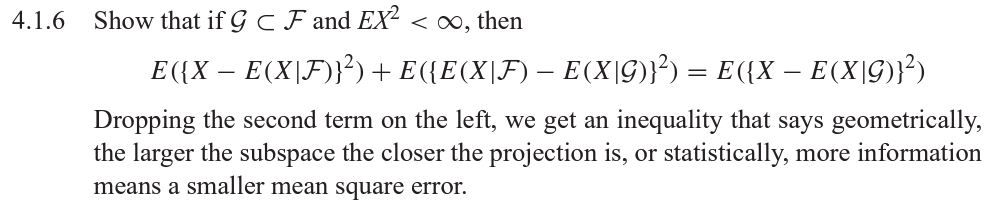
\includegraphics{Exer4.1.6.JPG}
\begin{remark}
	$E[\{X-E[X|\F]\}^2]\leq E[\{X-E[X|\G]\}^2]$ whenever $\G\subset \F$, provided $X\in \LL^2$ \\ The more information given, the closer to the target random variable in $\LL^2$ distance. 
\end{remark}
\begin{proof}
	\begin{multline*}
		E[\{X-E[X|\G]\}^2] = E[\{X-E[X|\F]+E[X|\F]-E[X|\G]\}^2] \\ = E[\{X-E[X|\F]\}^2]+E[\{E[X|\F]-E[X|\G]\}^2]+2E[\{X-E[X|\F]\}\{E[X|\F]-E[X|\G]\}]
	\end{multline*}
	Second equality holds because $X\in \LL^2 \Rightarrow E[X|\F], E[X|\G]\in \LL^2$ and $\LL^2$ is a vector space. Now, it suffices to show that the cross product $E[\{X-E[X|\F]\}\{E[X|\F]-E[X|\G]\}]$ is zero. We shall take advantage of a simple fact that $\G \subset \F \Rightarrow$ Every $\G$-measurable r.v. is $\F$-measurable. $\cdots (*)$
	\begin{align*}
		CP&=E[\{X-E[X|\F]\}\{E[X|\F]-E[X|\G]\}] \\
		&=E[E[\{X-E[X|\F]\}\{E[X|\F]-E[X|\G]\}|\F]]\quad \because E[Z]=E[E[Z|\F]] \\ &=E[\{E[X|\F]-E[X|\G]\}E[\{X-E[X|\F]\}|\F]] \quad \because E[X|\F]-E[X|\G]\in \F\; by\; (*) \\ &= E[0] \quad \because E[\{X-E[X|\F]\}|\F]=E[X|\F]-E[X|\F]E[1|\F]=E[X|\F]-E[X|\F]=0 \\ &= 0
	\end{align*}
	Therefore $E[\{X-E[X|\G]\}^2] = E[\{X-E[X|\F]\}^2]+E[\{E[X|\F]-E[X|\G]\}^2]$
\end{proof}
\vspace{1cm}

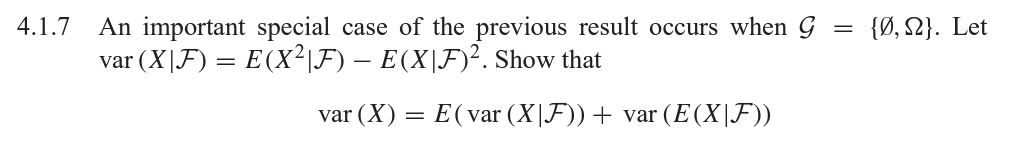
\includegraphics{Exer4.1.7.JPG}
\begin{remark}
	$Var(X|\F):=E[X^2|\F]-E^2[X|\F]=E[\{X-E[X|\F]\}^2|\F]$
\end{remark}
\begin{proof}
	Note that $E[X|\G]=E[X]$ when $\G=\{\phi, \Omega\}$. We shall plug in $\G=\{\phi, \Omega\}$ on the equation derived at problem 4.1.6
	\begin{enumerate}
		\item $E[\{X-E[X|\G]\}^2]=E[\{X-E(X)\}^2]=Var(X)$
		\item $E[\{X-E[X|\F]\}^2] = E[E[\{X-E[X|\F]\}^2|\F]]=E[Var(X|\F)]$
		\item $E[\{E[X|\F]-E[X|\G]\}^2] = E[\{E[X|\F]-E[X]\}^2]=E[\{E[X|\F]-E[E[X|\F]]\}^2]=Var(E[X|\F])$
	\end{enumerate}
	Problem 4.1.6 tells us that \romannumeral 1\; = \romannumeral 2 + \romannumeral 3. \;Thus $Var(X)=E[Var(X|\F)]+Var(E[X|\F])$
\end{proof}
\clearpage

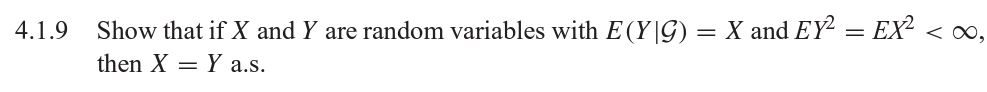
\includegraphics{Exer4.1.9.JPG}
\begin{proof}
	We again use the equation derived at problem 4.1.6 with plugging in trivial $\sigma$-field (which is a trick also used for problem 4.1.7)
	$$E[\{Y-E[Y|\F]\}^2] = E[\{Y-E[Y|\G]\}^2]+E[\{E[Y|\G]-E[Y|\F]\}^2]\quad whenever \;\F\subset \G,\; E[Y^2]<\infty$$
	Now plug in $\F=\{\phi,\Omega\}$. Then we have
	\begin{enumerate}
		\item $E[\{Y-E[Y|\F]\}^2]=E[\{Y-E[Y]\}^2]=Var(Y)$
		\item $E[\{Y-E[Y|\G]\}^2]=E[\{Y-X\}^2]$
		\item $E[\{E[Y|\G]-E[Y|\F]\}^2]=E[\{X-E[Y]\}^2]$
	\end{enumerate}
	Thus we have $Var(Y)=E[\{Y-X\}^2]+E[\{X-E[Y]\}^2]\;\cdots\;(\star)$ \\
	Notice that $E[X]=E[E[Y|\G]]=E[Y]$. $(\star)$ turns to $Var(Y)=E[\{Y-X\}^2]+Var(X)$. \\Since $E(X)=E(Y)$ and $E(X^2)=E(Y^2)<\infty$ by assumption, we have $Var(X)=Var(Y)<\infty$ \\ Therefore, we get $E[\{Y-X\}^2]=0$. It implies that $(Y-X)^2=0 \;\; a.s.\quad \because (Y-X)^2\geq 0$ \\ Thus $|Y-X|=0\;\; a.s.$ and $X=Y \; a.s.$
\end{proof}



\end{document}